
\chapter{Methodology}
To answer \textbf{RQ1} we develop, train and evaluate a model conditioned with inner metric weight. \textbf{RQ2} and \textbf{RQ3} are both answered using a user study that collects metrics on player interactions with the music alongside survey responses. 

\section{The Model}
Sections \ref{section:non_neural_generation} and \ref{section:deep_learning_generation} discussed the potential approaches to music generation with particular attention to state of the art approaches using deep learning. The developed model will be a transformer due to its ability to effectivley model sequences whether it be language or music as well as its potential to incooperate additional controls. We will be using a symbolic representation of music (as discussed in section \ref{section:symbolic_audio}) due to its lightweight datasets and the ability to make changes and incooperate the output into a music production environment, enabling a cooperative co-composition process as opposed to replacing the composer. More specifically we will be using a representation similar to REMI+ (see section \ref{section:symbolic_tok}), a representation that extends the standard MIDI-events with tokens indicating form, such as meter, bar-lines and note-duration. This representation will be compounded using byte pair encoding (see section \ref{section:symbolic_tok}) to decrease the sequence length and improve the capability and efficienty of the model. For adding control (section \ref{section:addingcontrol}) we will focus on methods that don't require full training, specifically parameter efficient fine tuning and and guidance. This is more cost-effective and environmentally friendly. We will use the Lakh Midi Dataset \cite{Raffel_2016}, a widely used open source and licensed dataset for symbolic music generation. This will help us avoid ethical pitfals around privacy and copyright. (section \ref{ethical}). Finally. we are not attempting to add control by training custom large foundation models, rather we are using parameter efficient fine tuning or guidance (section \ref{section:addingcontrol}) to add contro. As a result we are using no or only a fraction of the model parameters, with substantially less need for data, computation, and energy. All relevant code, including code for training, configuration and data-preparation will be made available online alongside the model weights. Finally I use and extend an open-source model MusicLang in collaboration with it's maintainers. If successfull theese extensions will contribute to the MusicLang project and be widely available in a well documented and continously maintained ecosystem, with integrations into mainstream music production and composition software. 

\section{Developing the Model}

\subsection{Preliminary Experiments - proof of concept}
The current methods of adding musical control to an existing model are poorly systemetized and rarely compared to each other. While this thesis does not aim to provide a systemic comparison and experimental evaluation of different control methods, some preliminary experiments are necessary to establish the best course of action. We use BassCraft a smaller model, and start by controlling for note-density (the number of notes in a bar), a feature that is more easily calculated, tokenized and verified as opposed to inner metric weight.  

\subsubsection{BassCraft -  a tiny transformer model}
To avoid wasting valuable compute resources and energy we perform the preliminary experiments on a smaller model: Basscraft. BassCraft is a small transformer model based on  GPT2 \cite{Radford_Wu_Child_Luan_gpt2_2019}. It has an embedding size of 256, 4 attention heads, 4 hidden transformer layers, and a total of 7 million trainable parameters. For contrast the target LLAMA 2 based model MusicLang has over 100 million trainable parameters. Basscraft is trained to generate a bassline to a provided piece of music using the lakh-midi dataset \cite{Raffel_2016}. For training, songs with bass-lines are selected (based on the presence of particular MIDI-instrument channels). The tracks are partitioned into snippets between 1 and 16 bars long. The bass-lines are separated from the remaining track and matched as potential output. 

\begin{figure}[H]
    \centering
    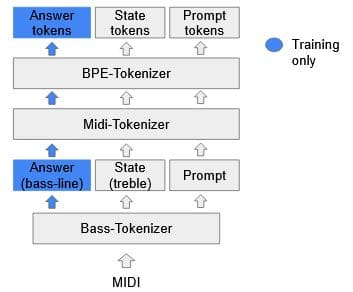
\includegraphics[width=0.5\textwidth]{IMAGES/Preprocessing1.jpg} 
    \caption{Preprocessing/tokenization of the original basscraft model}
    \label{fig:preprocessing1}
\end{figure}

\subsubsection{Fine-Tuning 1 - Vocabulary Extension}

Vocabulary expansion is the process to add new vocabulary to a transformer model. MusicLang achieves it's extraordinary controlability similarly to FIGARO \cite{Rütte_figaro_2023} using control tokens, that summarize features of the music that go beyond simply representing MIDI-events. In vocabulary extension it is critical to ensure that additional tokens do not overwrite or otherwise collide with the existing training, otherwise the benifit of using a priorly trained model is eliminated. Since we are using a BPE tokenizer, is difficult to simply add new tokens here, as it would require retraining the BPE tokenizer, which will transform the embedding layer making the entire model unusable. Instead we investigate whether there are unused tokens, and reassign them to our new control tokens. Theese new tokens will not be included in any of the coumpound tokens generated by the BPE process, which does negativley effect the sequence length.

\begin{figure}[H]
    \centering
    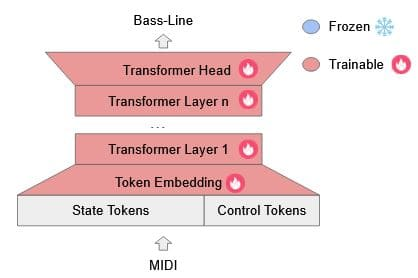
\includegraphics[width=0.5\textwidth]{IMAGES/full_ft.jpg}
    \caption{Vocabulary transfer with full fine tuning}
    \label{fig:vocabtrans1}
\end{figure}

\begin{figure}[H]
    \centering
    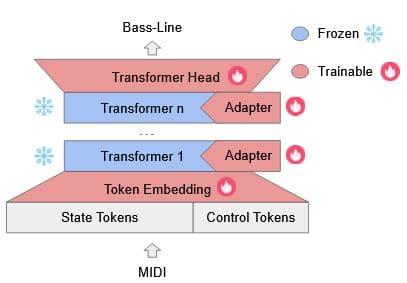
\includegraphics[width=0.5\textwidth]{IMAGES/vocab_lora_ft.jpg} 
    \caption{Vocabulary transfer with parameter efficient fine tuning}
    \label{fig:vocabtrans2}
\end{figure}

\subsubsection{Fine-Tuning 2 - Integrating of control tokens} 

This approach is slightly different from the vocabulary extension, because it processes the additional control tokens as a paralell stream. This is similar to the the approach used in Coco-Mulla \cite{Lin_cocomulla_2024}. The paralell stream of control tokens is inserted into the model after c layers (with bypasses that insert the embedding into every following layer), after passing through a custom learned embedding. The benifit of this method is that it doesn't require editng the model's vocabulary. 
 
\begin{figure}[H]
    \centering
    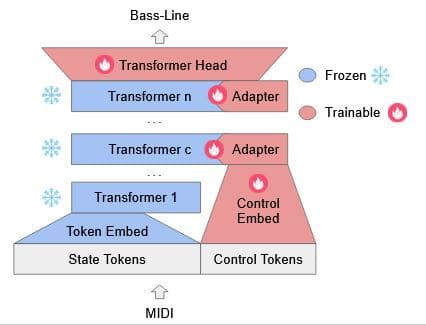
\includegraphics[width=0.5\textwidth]{IMAGES/ControlTokensLora.jpg} 
    \caption{Integration of control tokens with parameter efficient fine tuning}
    \label{fig:controltok}
\end{figure}

\subsubsection{Post-Hoc Guidance and other improvements}

This is the approach used by SMITIN\cite{Koo_Wichern_Germain_SMITIN_2024}. This type of sampling based guidance has been very successfull in diffusion models, however in transformers it produces mixed results \cite{language_guide_rutte_2024}.  One potential problem: This may be very difficult to implement. Both SMITIN and Rütte\cite{language_guide_rutte_2024} only use one dimensional variables (probability of a concept being present or not).

\begin{figure}[H]
    \centering
    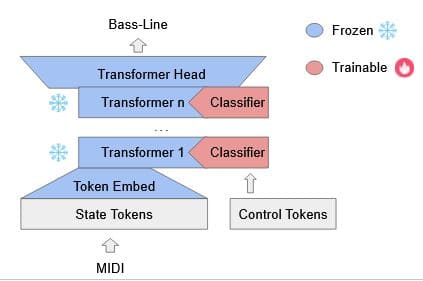
\includegraphics[width=0.5\textwidth]{IMAGES/adhoccontrol.jpg} 
    \caption{Integration of control using inference time interference}
    \label{fig:adhoccontrol}
\end{figure}

If these experiments are not successful, we can follow the approach of \cite{Shu_Xu_Musebarcontrol_2024} and try additional training using auxiliary tasks and using a modified (counterfactual) loss function. 


\subsection{MusicLang - The foundation Model}
After concluding the preliminary experiments and identifying a promising set of methods. We will proceed with the larger MusicGen model. 
MusicLang's core model is a transformer based on LLAMA 2 trained on the Lakh Midi Dataset\cite{Raffel_2016}. It can generate relativley long multi-track instrumental pieces, (a couple of minutes) with control for chord progression, instrumentation and range. Additionally it can generate interpolations and continuations of a user provided piece. It is trained on an extended vocabulary of tokens similar to REMI\footnote{https://musiclang.github.io/tokenizer/} with additional tokens detailing harmonic structure and voice characteristics i.e instrumentation or range (see figure \ref{fig:musiclangtok}). This base vocabulary is additionally extended using the BPE tokenizer. The goal of this section is to extend MusicLang with control for inner metric weight.  

\begin{figure}[H]
    \centering
    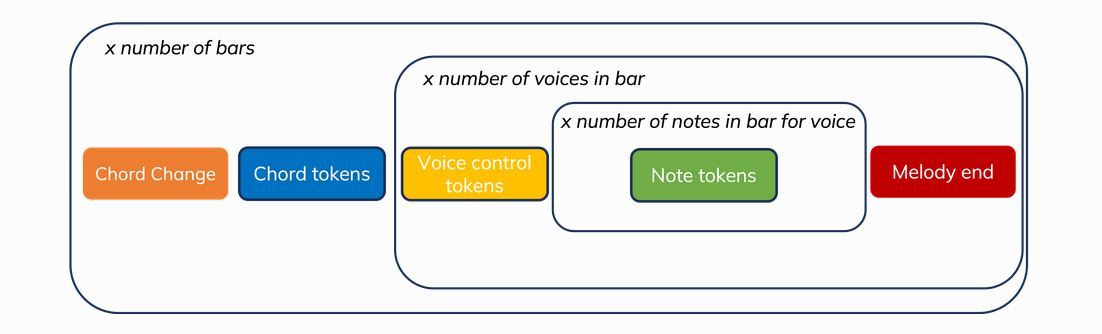
\includegraphics[width=0.5\textwidth]{IMAGES/MusicLang.JPG} 
    \caption{MusicLang tokenisation on a high level}
    \label{fig:musiclangtok}
\end{figure}

\subsection{Using inner metric weight as controlable feature}
Inner metric analysis (IMA) creates metric weight profiles which we use as guiding feature passed to the model bar by bar, which allows us to induce shifts in metric weight in the output. 
For this we use the globally smallest available note grid of the lakh-midi dataset $g_min$. Theese distributions are normalized and provided to the model as vectors of length $g_{min}$.
The model then learns embeddings of the distribution alongside positional embeddings \cite{Lin_cocomulla_2024}. Theese embeddings are then added to the model starting from a certain stop.
For inference the user can provide a reference track from which the inner metric profile is extracted and then passed to the model. 
\begin{figure}[H]
    \centering
    \begin{subfigure}{0.45\textwidth}
        \centering
        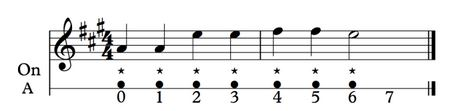
\includegraphics[width=\linewidth]{IMAGES/IMA1.JPG}
        \caption{Single local meter and its pulses (A) from the melody "Twinkle, Twinkle Little Star"}
        \label{fig:ima1}
    \end{subfigure}
    \begin{subfigure}{0.45\textwidth}
        \centering
        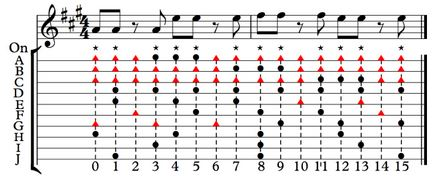
\includegraphics[width=\linewidth]{IMAGES/IMA2.JPG}
        \caption{10 local meters and their pulses produced by IMA of a syncopated variation of "Twinkle, Twinkle Little Star"}
        \label{fig:ima2}
    \end{subfigure}
    
    \vspace{0.5cm} % Adjust spacing between rows

    \begin{subfigure}{0.45\textwidth}
        \centering
        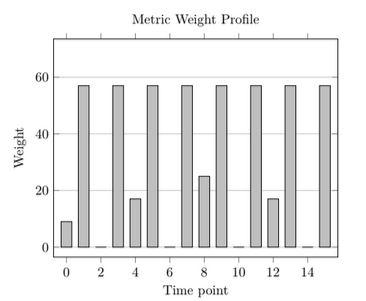
\includegraphics[width=\linewidth]{IMAGES/IMA3.JPG}
        \caption{Metric weight profile of syncopated "Twinkle, Twinkle Little Star"}
        \label{fig:ima3}
    \end{subfigure}
    \begin{subfigure}{0.45\textwidth}
        \centering
        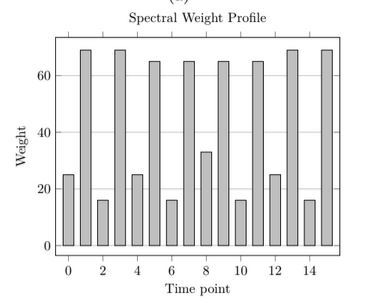
\includegraphics[width=\linewidth]{IMAGES/IMA4.JPG}
        \caption{Spectral weight profile of syncopated "Twinkle, Twinkle Little Star"}
        \label{fig:ima4}
    \end{subfigure}

    \caption{Visualisation of metric weight analysis \cite{Bemman2024}}
    \label{fig:ima_all}
\end{figure}


\subsection{Evaluating Control-Effectivness}
As discussed in section \ref{section:evaluation}, calculating whether or not the control is effective, depends on the controlled feature, but can happen automatically. \\
For the preliminary experiments targeting note density this can be done as follows, if note density is measured as a categorical variable i.e low, medium, high, the error would be calculated similarly to a multilabel classifier, where the predicted is label is the note_density of the generated music, and the true label is the note_density given in the prompt on a bar by bar level. The metrics inlcude accuracy, precision, recall and F1 scores If note-density is continuous (i.e notes per bar), then the error would be calculated as mean square error. \\
\[
error_{continuous} = \sqrt{\frac{1}{n}\sum_{j=1}^{n}(y_{generated}-y_{prompt})}
\]
Inner metric weight analysis generates metric weight profiles, which we use as guidance mechanism. Following the approach by \cite{Bemman2024} we can compare the the generated and the target rhythmic weight profiles using chi-squared distance.
Given target distribution $T$ and generated distribution $G$ the distance is given by 
\[
D=\sum_{i=0}^{n-1}\left(\frac{(T_i-G_i)^2}{T_i+G_i}\right)
\]

\section{User Study}
\textbf{RQ2} and \textbf{RQ3} are evaluated through a user study. The goal is too recruit $n=20$ participants to complete an interactive test of interactability and a survey comparativley evaluating the generated music. 
\subsection{Interactive Study}
The interactive study aims to evaluate the fittness of the controlled generated music from an MACT perspective. Specifically, in the MACT protocoll used by Chalkiadakis \cite{Chalkiadakis_2022}, the patient is supposed to listen to changes in the music, and change their playing. In our simplified interactive sessions the player is asked to hit a button whenever they hear a change in the music. The button-presses are registered alongside the starting time, tempo and registered changing points (determined from the prompt). Finally, the timing of the button presses and registered changes is correlated with each other. High correlation indicates that the participants noticed the changes. 

\subsection{Survey}
The survey will compare the listening experience of different symbolic generative models including our model, FIGARO \cite{Rütte_figaro_2023} and Polyfussion \cite{Min_Jiang_Xia_Zhao_polyffusion_2023} as well as the improved rule based generator of "Last Minute Gig" \cite{Chalkiadakis_2022}\cite{Schlette_2022}. 
The questionnaire will include questions on personal details of the participant, gender, age, educational background, musical experience and gaming experience.

\section{Thesis Timeline}

\begin{figure}[H]
    \centering
    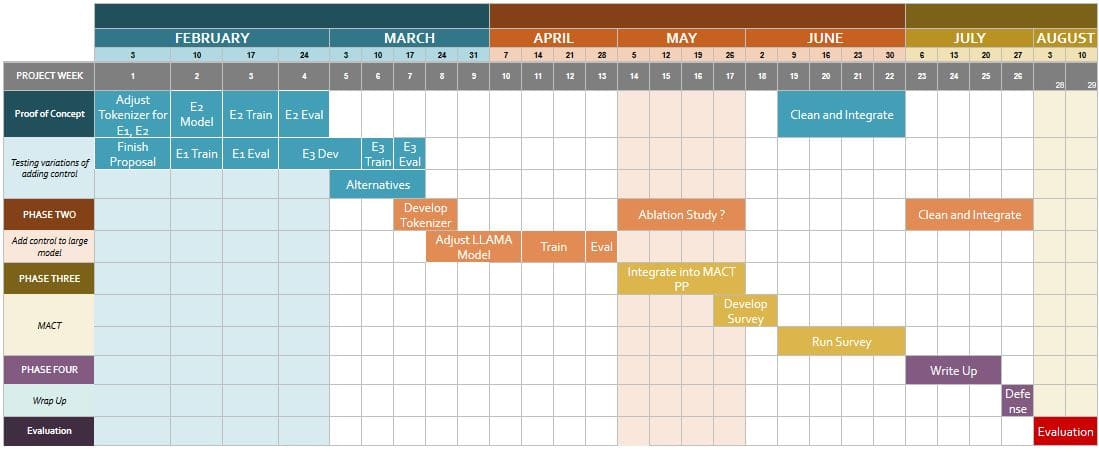
\includegraphics[width=1\textwidth]{IMAGES/project_plan.jpg} 
    \caption{Thesis project plan}
    \label{fig:projectplan}
\end{figure}


